\documentclass[11pt,letterpaper]{article}
\usepackage{graphics}
\usepackage{fullpage}
\addtolength{\voffset}{0.5in}

%
%  Cool LaTeX resource:
%   http://en.wikibooks.org/wiki/LaTeX

\begin{document}
\title{Self-improving tutor system}
\author{Brett van de Sande}

% Assignment of blame paper: 
% http://www.public.asu.edu/~kvanlehn/Stringent/PDF/07UM_KVL_KK_etal.pdf
%   my ``opportunity'' equals their ``step''
%   my ``turn'' equals their ``transaction''
%
% Doing reinforcement learning by direct policy search.
% See discussion on p. 17 of:
% http://www.cs.brown.edu/research/pubs/theses/phd/2002/peshkin.pdf


\maketitle

\section{A model of learning}

For each student and KC, the student has attempted some number of 
{\em steps} that involve a given skill.   We will label
steps with $j$.  Usually a given step is associated
with a single user interface object (an equation, vector, etc.)  but
not always, since a student may attempt a particular problem solving
step, delete the object, and later attempt that solution step again.
Each step $j$ corresponds some some number of student {\em transactions}:
attempts at constructing the associated object, or associated
interactions with the Andes help system.  

Next, we need of student learning for a particular KC.
Since the policies chosen by the random-help version of Andes
are different for each student,
we need to determine the point of learning for each student.
For each KC and student, mark each step as ``correct'' if
the student completes the step correctly without any associated errors or 
requests for help; otherwise, the step is marked as ``incorrect.''


\section{Objective function}

The basic appoach for solving this problem, in terms of reinforcement
learning, is called a ``direct policy search.''
For each student, help-giving policy, and KC, we define the objective 
function to be 
%
\begin{eqnarray}
  Z &=& \sum_{j \in \mathcal{I},L>j}  
  % Actually, we use the number of incorrect steps
  % between j and L for the discount factor.
  % need to add this to formula.
       \frac{\gamma^{n(L,j)-1} w_L \Delta_L}{\left|\sigma_j\right|}
  \sum_{k\in \sigma_j} \left(f(\mathbf{x}_k)-d_k\right))^2 \nonumber \\
 % reward for after-learning policy
 % Includes case with no learning as k=0.
  &&+\beta \sum_{j \in \mathcal{I},L \le j} \frac{(1-P(S)) w_L}
      {\left(\left|\matchal{I}\right|-L\right)\left|\sigma_j\right|}
             \sum_{k\in \sigma_j} \left(f(\mathbf{x}_k)-d_k\right))^2
\end{eqnarray}
%
where  $\mathcal{I}$ is the set of incorrect steps associated
with that student, policy, and KC when the model has detected 
learning.  Also, $n(L,j)$ is the number
of $\mathcal{I}$ between $L$ and $j$, $w_L$ is the probability 
that the student learned the skill at step $L$, $\Delta_L$ is the learning
gain $1-\left\langle g+s \right\rangle$ at step $L$, and $\gamma$ 
is the ``discount factor''\cite{ml}.  
$\sigma_j$ is the set of transactions associated with step $j$ and
$d_k\in \{0,1\}$ is the
policy actually taken by the random-help version of Andes for transaction
$k$,
We have arranged things so that finding an optimal policy 
corresponds to {\em minimizing} $Z$.


\section{Models of learning}

A number of authors have used a logistic funtion, 
$\mathrm{logit}(x)=(1+\tanh(x/2))/2$, to 
model student learning.  In that case, we have a two-parameter
model for the probability that the student gets step $j$ correct:
%
\begin{equation}
               P_j^\mathrm{logit} = \mathrm{logit}\left(\beta (j-L)\right)
\end{equation}
%
where $\beta$ is the learning rate and $L$ is the ``moment
of learning''~\cite{aha}.

Alternatively, we can use a function that retains the 
guess $P(G)$ and slip $P(S)$ probabilities of Corbett and 
Anderson~\cite{anderson}.
The simplest such model is a step-function:
%
\begin{equation}
               P_j^\mathrm{step} = \left\{\begin{array}{cc}
                                       g,& j<L\\
				       1-s,& j\ge L
                                    \end{array}\right. \label{step}
\end{equation}
where $g$ is the guess rate, $s$ is the slip rate and 
$L$ is the moment of learning.
%
\[
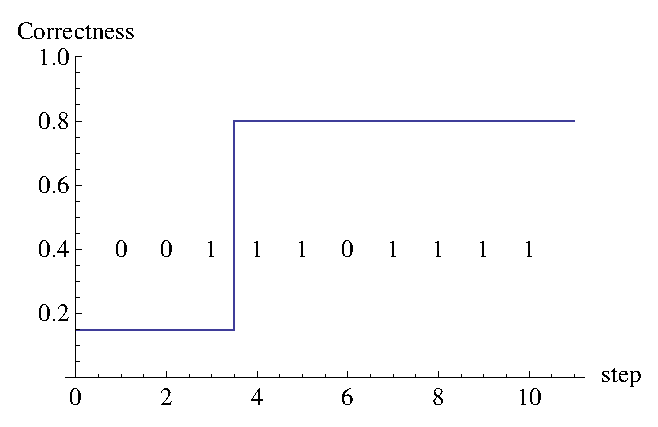
\includegraphics{step.eps}
\]
%
We can match $P_j^\mathrm{step} $ to the student data using the
Maximun Likelihood method.
Let $c_i$ \& $w_i$ be the number of correct \& incorrect steps observed
for steps $j<L$ and $c_f$ \& $w_f$ be the number of correct \& incorrect
steps for steps $j\ge L$.  The associated log likelihood for a given $L$ is
%
\begin{equation}
  \mathcal{L}_L  =  \log\left(B_{c_i,w_i}(g)\right) 
                      + \log\left(B_{c_f,w_f}(1-s) \right)  \, ,
\end{equation}
%
where the guess rate $g$ and slip rate $s$ follow the binomial distribution,
%
\begin{equation}
       B_{a,b}(x) = x^a (1-x)^b\; \frac{(x+b+1)!}{a!\, b!} 
      \;\;\;\; \mbox{where} \;\;\;\;
      1=\int_0^1 B_{a,b}(x) \,\mathrm{d}x \; .
\end{equation} 
%
$\mathcal{L}_L$ is maximized when:
%
\begin{eqnarray}
  g = P(G) &=&  \frac{c_i}{c_i+w_i} \, ,\\
  s = P(S) &=&  \frac{w_f}{c_f+w_f} \,  .
\end{eqnarray}
%
Next, one can maximize $\mathcal{L}_L$ with respect to $L$ to find
the most likely value $L=L_\mathrm{max}$.  However, in practice, the 
uncertainty in $L$ can be significant and may not have a normal
distribution.   Instead, we will consider a set of sub-models, each with a 
different value of $L$, and a relative probability given by 
AIC~\cite{aic-book}.  
That is, the sub-model for a particular value of $L$ has weight,
%
\begin{equation}
                   w_L = \frac{\mathrm{e}^{\mathcal{L}_L-2} }{W}\, ,
\end{equation}
%
with normalization $W$ such that $\sum_L w_L=1$.
For each sub-model, we can define an averag learning gain,
%
\begin{equation}
     % need actual formula here.
         \Delta_L = 1- \left\langle g+s \right\rangle \; .
\end{equation}

Finally, we need to determine whether, in the context
of the step-function model (\ref{step}), learning has occurred.
We say that learning has occurred at $L$ if $g<1-s$.
Since the model is a fit to student data ($c_i$, $w_i$, $c_f$, $w_f$), 
we can, at best, determine the {\em probability} that learning has occurred. 
The probability that learning has occurred can be calculated by
integrating over the possible slip and guess rates in the region
$p+g<1$, weighted by the probability distributions:
%
\begin{equation}
   P(c_i, w_i, c_f, w_f)= \int_0^1 \int_0^{1-g} 
   B_{c_i,w_i}(g) \, B_{c_f,w_f}(1-s) \,\mathrm{d}g\,\mathrm{d}g 
\end{equation}
%
This integral can be solved by repeated integration by parts,
giving:
%
\begin{equation}
   P(c_i, w_i, c_f, w_f)= \mbox{long formula here} \; .
\end{equation}




\begin{thebibliography}{9}

\bibitem{anderson} 
  Corbett, A.\ T., Anderson, J.\ R. Knowledge Tracing:  Modeling 
the Acquisition of Procedural Knowledge.  \emph{User Modeling and
 User-Adapted Interaction}, 1995, 4, 253--278.

\bibitem{beckchang}
  Beck, J.\ E., Chang, K.-m.\ Identifiability: A Fundamental Problem of
  Student Modeling.
  \emph{Proceedings of the $11^{th}$ International Conference on User 
    Modeling}, 2007.

\bibitem{aic-book}Burnham, K.~P., and Anderson, D.~R. \emph{Model
  Selection and Multimodel Inference: A Practical
  Information-Theoretic Approach}, 2nd ed. Springer-Verlag. 2002.

\bibitem{aha}Kurt and Kasia moment of learning paper.

\bibitem{ml}Discount factor citation.

\end{thebibliography}




\end{document}